\documentclass{article}

\usepackage{listings}
\usepackage{enumitem}
\usepackage{amsmath}
\usepackage{svg}
\usepackage{hyperref}
\hypersetup{
    colorlinks=true,
    linkcolor=blue,
    filecolor=magenta,      
    urlcolor=cyan,
    pdftitle={Overleaf Example},
    pdfpagemode=FullScreen,
    }

\title{CA Lab: Homework 7}
\author{student: Dimitri Tabatadze}

\newcommand{\points}[1]{{\footnotesize{\color{red}\textit{#1 points}}}}

\definecolor{codegreen}{rgb}{0,0.6,0}
\definecolor{codegray}{rgb}{0.5,0.5,0.5}
\definecolor{codepurple}{rgb}{0.58,0,0.82}
\definecolor{backcolour}{rgb}{0.98,0.96,0.94}

\lstdefinestyle{mystyle}{
    backgroundcolor=\color{backcolour},   
    commentstyle=\color{codegreen},
    keywordstyle=\color{magenta},
    numberstyle=\tiny\color{codegray},
    stringstyle=\color{codepurple},
    basicstyle=\ttfamily\footnotesize,
    breakatwhitespace=false,         
    breaklines=true,                 
    captionpos=b,                    
    keepspaces=true,                 
    numbers=left,                    
    numbersep=5pt,                  
    showspaces=false,                
    showstringspaces=false,
    showtabs=false,                  
    tabsize=2
}

\lstset{style=mystyle}

\begin{document}
    \maketitle

    \section*{Task Description} 
    
    {General Purpose Register Drawing}



    \begin{enumerate}
        \item Size of addresses: If we have 32 registers, what should be size of address bus (\verb|addrA|/\verb|B|)?
        \item Read Registers: Draw a rectangle, representing register file and attach inputs and outputs to it. Also indicate size (number of bits) of inputs and outputs on your drawing.
        \item Register \verb|0|: In your drawing implement digital circuit that makes sure that register \verb|$0| stays \verb|0| all the time.
    \end{enumerate}

    \section*{Solution}

    \begin{figure}[h]
        % \caption{}
        \begin{center}
            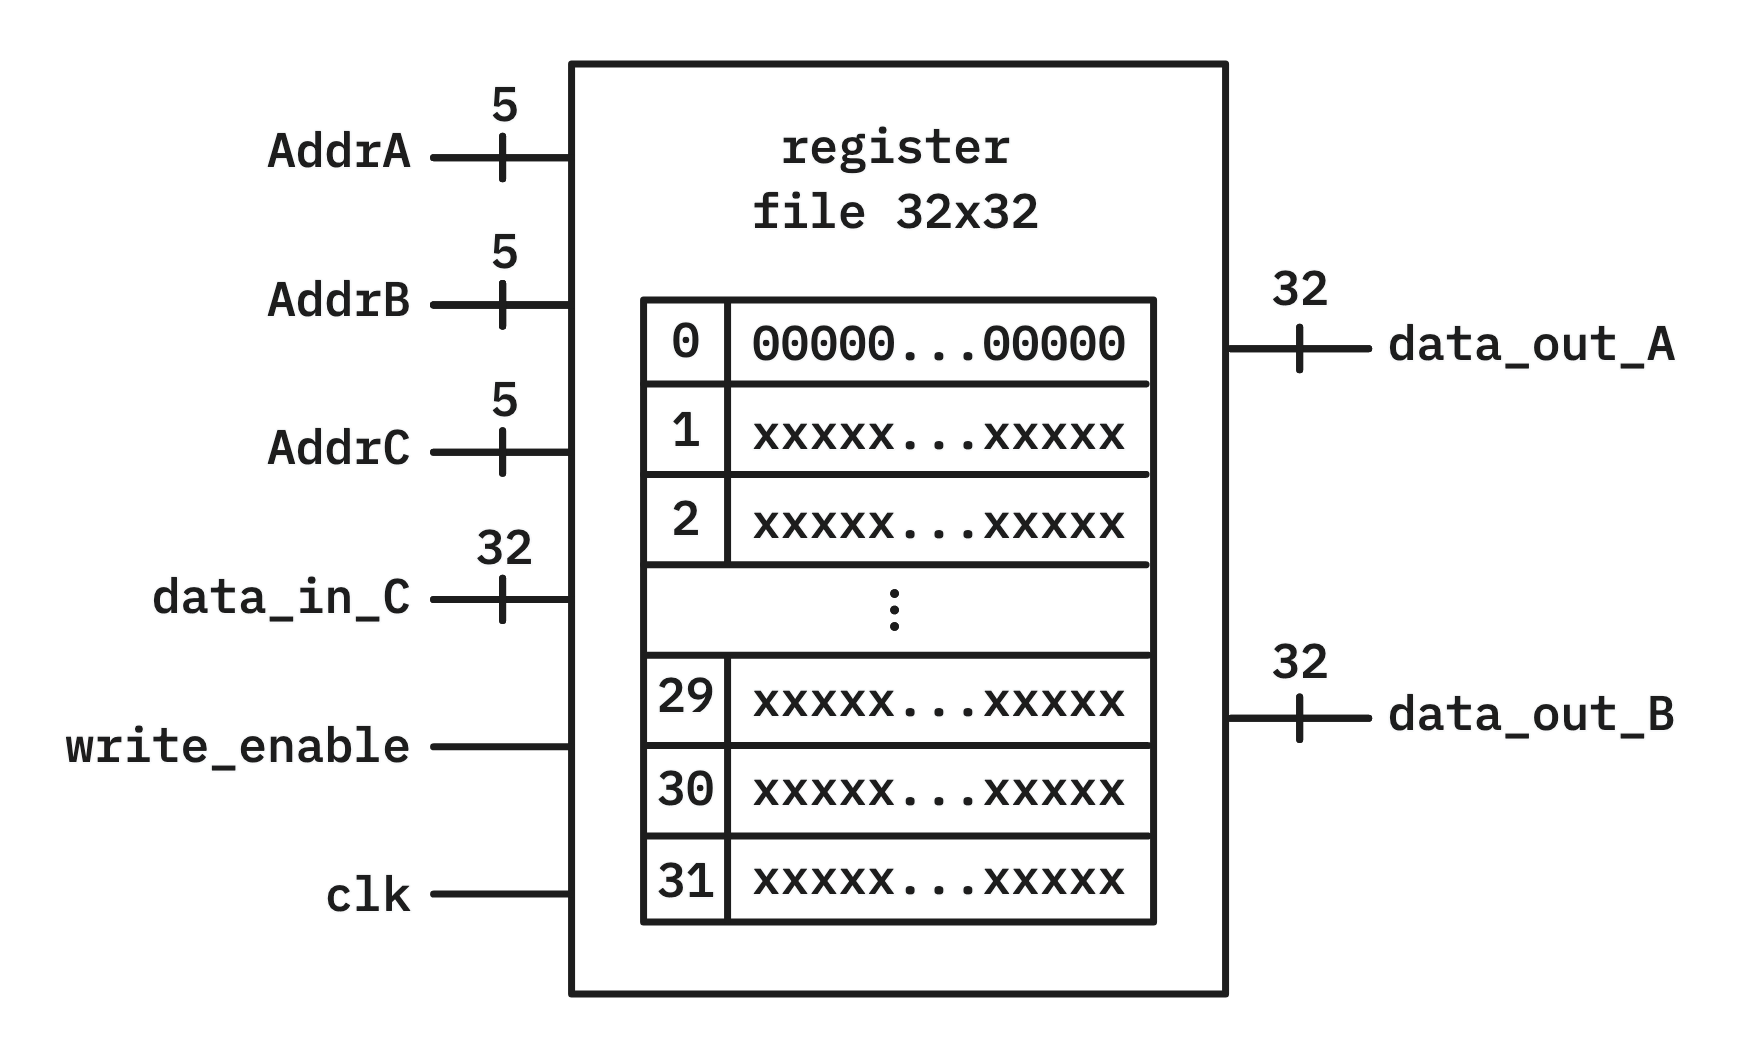
\includegraphics[width=8cm]{shapes.png}
        \end{center}
    \end{figure}

    \section*{Reference}
    
    \begin{itemize}
        \item me.
    \end{itemize}

\end{document}